\documentclass[xcolor=dvipsnames,compress,10pt]{nersc}
\lstdefinestyle{OpenMP-directive} {language=C, style=numbers, style=MyFrame, frame=lines, style=MyFontStyle}
\usepackage{fancybox}
\usepackage{subcaption}
\usepackage{listings}
\usepackage{adjustbox}
\usepackage{array}
\usepackage{graphicx}

%%%%%%%%%%%%%%%%%%%%%%%%%%%%%%%%%%%%%%%%%%%%%%%%%%%%%%%%%%%%%%%%%%%%%%%%%%%%%%%%

\title[Short Title]{Unifying OpenMP offload support}
\subtitle{}
\author[Rahul Gayatri]{\Large Rahulkumar Gayatri}
\meeting{Performance Portability Meeting 2019, Denver}

%%%%%%%%%%%%%%%%%%%%%%%%%%%%%%%%%%%%%%%%%%%%%%%%%%%%%%%%%%%%%%%%%%%%%%%%%%%%%%%%
%
\begin{document}

%------------------------------------------------------------------------------%
%
\begin{frame}[label=title,plain]
    \maketitle
\email{rgayatri@lbl.gov}
\end{frame}

%%%%%%%%%%%%%%%%%%%%%%%%%%%%%%%%%%%%%%%%%%%%%%%%%%%%%%%%%%%%%%%%%%%%%%%%%%%%%%%%
\section{Motivation for the work}
\begin{frame}{OpenMP to target GPUs}
\begin{itemize}
    \setlength\itemsep{1.2em}
    \item 5 of top 10 supercomputers are GPU based machines
    \begin{itemize}
        \item Most of the codes optimized for CPUs have to now
            be rewritten to take advantage of the graphics card
    \end{itemize}
    \item OpenMP~4.5 supports GPU offloading
    \begin{itemize}
        \item Port incrementally for big codes
        \item Control the parallelization via compile time flags
        \item Need not be concerned with optimizations for newer architectures
    \end{itemize}
    \item Bottleneck - Find compilers that support OpenMP~4.5
\end{itemize}
\end{frame}

%%%%%%%%%%%%%%%%%%%%%%%%%%%%%%%%%%%%%%%%%%%%%%%%%%%%%%%%%%%%%%%%%%%%%%%%%%%%%%%%
\section{Motivation for the talk}
\begin{frame}{Why Attend this Talk}
\begin{enumerate}
    \setlength\itemsep{1.2em}
    \item OpenMP~4.5 directives
    \item This talk would provide a detailed analysis of the current state of OpenMP~4.5 implementations
    \begin{itemize}
        \item Supported compilers
        \item Differences in compiler implementations
    \end{itemize}
    \item Performance portability
    \begin{itemize}
        \item Interpretations of OpenMP~4.5 directives on CPUs
    \end{itemize}
\end{enumerate}
\end{frame}

%%%%%%%%%%%%%%%%%%%%%%%%%%%%%%%%%%%%%%%%%%%%%%%%%%%%%%%%%%%%%%%%%%%%%%%%%%%%%%%%%
%\section{Overview}
%\begin{frame}{Outline of the Presentation}
%\begin{itemize}
%    \setlength\itemsep{1.5em}
%    \item OpenMP~4.5 directives
%    \item Differences in Compiler mapping of directives on GPU hardware
%    \item Interpretation of OpenMP~4.5 directives on CPUs
%\end{itemize}
%\end{frame}

%%%%%%%%%%%%%%%%%%%%%%%%%%%%%%%%%%%%%%%%%%%%%%%%%%%%%%%%%%%%%%%%%%%%%%%%%%%%%%%%
\section{GPU Programming Models}
\subsection{OpenMP~4.5 }
\begin{frame}[fragile] {OpenMP offloading to GPU}
\begin{center}
\end{center}
\begin{columns}[t]
\begin{column}{.38\textwidth}
\begin{itemize}
    \setlength\itemsep{1.5em}
    \item OpenMP~4.5 compilers
    \begin{itemize}
        \item XL/16.1(IBM)
        \item Clang - LLVM-9.0
        \item GCC/8.1
        \item Cray/6.0
    \end{itemize}
\end{itemize}
\end{column}
\begin{column}{.58\textwidth}
\shadowbox{Volta GPU available on Cori and Summit}
\begin{center}
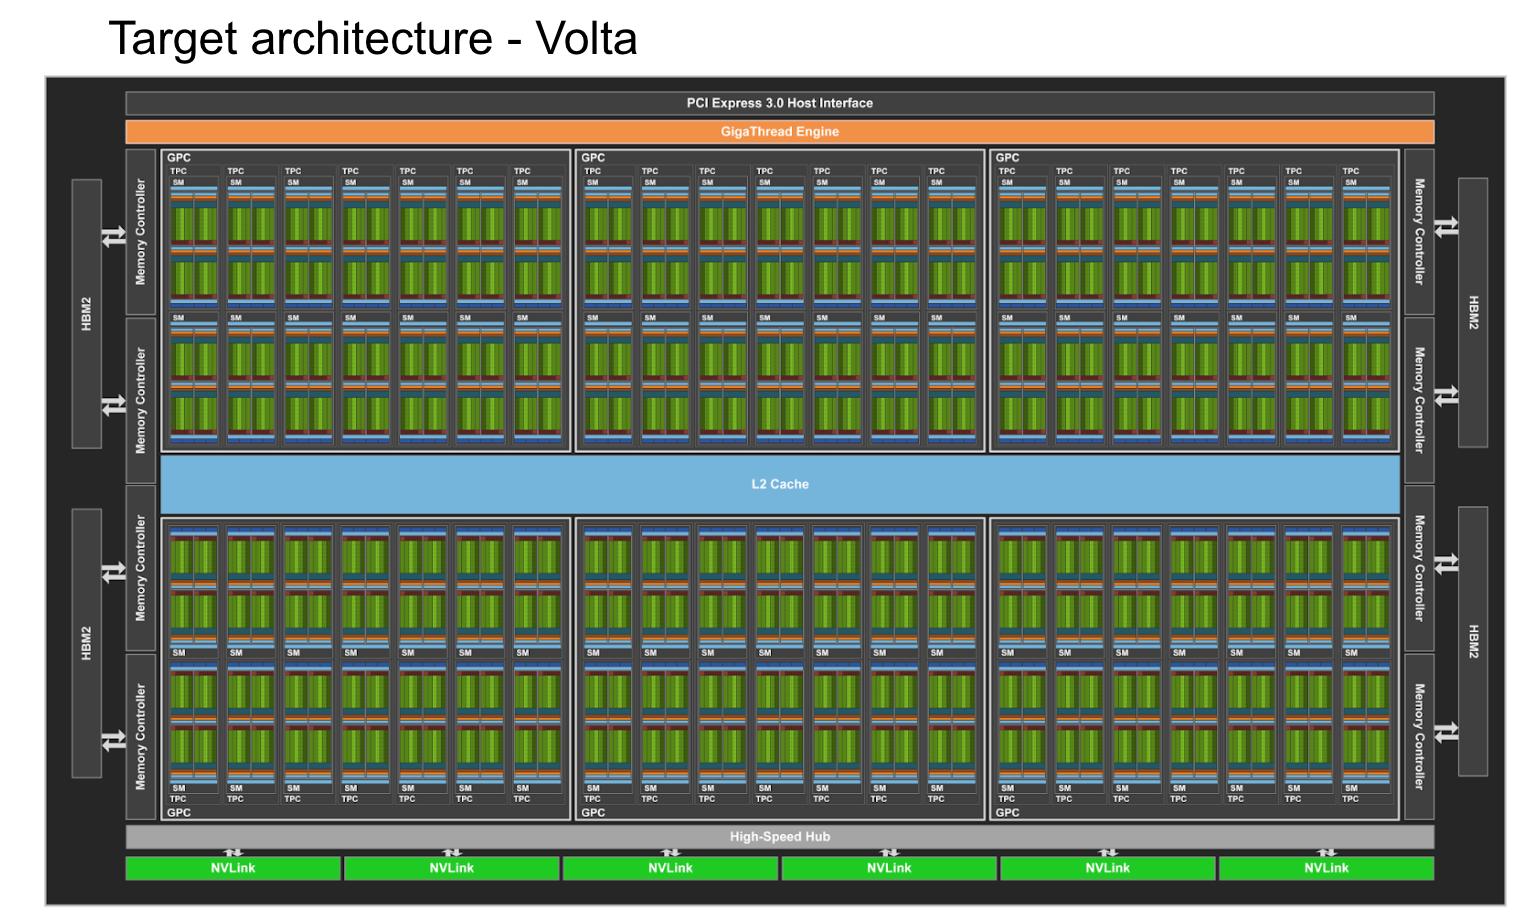
\includegraphics[width=\linewidth]{images/volta_architecture.png}
\end{center}
\end{column}
\end{columns}
\end{frame}

\sectiontransitionslide{OpenMP~4.5 directives}

%%%%%%%%%%%%%%%%%%%%%%%%%%%%%%%%%%%%%%%%%%%%%%%%%%%%%%%%%%%%%%%%%%%%%%%%%%%%%%%%
\section{OpenMP~4.5 Offload Directives}
\begin{frame}[fragile]{OpenMP directives to offload code-blocks onto GPUs}
\shadowbox{Directives to distribute work across GPU threads}
\begin{lstlisting}[style=cleanText]

#pragma omp target //offload code block onto GPU-accelerator
{
    #pragma omp teams distribute //Distribute across threadblocks
    for()
    {
        #pragma omp parallel for simd//Distribute across threads
        for()
        {
        }
    }
}

\end{lstlisting}
\end{frame}

%%%%%%%%%%%%%%%%%%%%%%%%%%%%%%%%%%%%%%%%%%%%%%%%%%%%%%%%%%%%%%%%%%%%%%%%%%%%%%%%
\section{OpenMP~4.5 Data Movement}
\begin{frame}[fragile]{Directives to move data to/from device/host}
%
\shadowbox{Clauses to use with \textcolor{red}{\textbf{target}} directives}
\begin{lstlisting}[style=cleanText]
map(to:...) <@\hspace{5mm}@> map(from:...) <@\hspace{5mm}@> map(tofrom:...)
\end{lstlisting}
%
\shadowbox{Allocate and delete data on the device}
\begin{lstlisting}[style=cleanText]
#pragma omp target enter data map(alloc: list-of-<@\textcolor{blue}{data}@>-structures[:])
#pragma omp target exit data map(delete: list-of-<@\textcolor{blue}{data}@>-structures[:])
\end{lstlisting}
%
\shadowbox{Update data on device and host}
\begin{lstlisting}[style=cleanText]
#pragma omp target update to/from (list-of-<@\textcolor{blue}{data}@>-structures[:])
to - HostToDevice
from - DeviceToHost
\end{lstlisting}
\end{frame}

%%%%%%%%%%%%%%%%%%%%%%%%%%%%%%%%%%%%%%%%%%%%%%%%%%%%%%%%%%%%%%%%%%%%%%%%%%%%%%%%
\section{OpenMP~4.5 Routines on Device}
\begin{frame}[fragile]{OpenMP~4.5 directives to offload routines on the device}
\shadowbox{Routines}
\begin{lstlisting}[style=cleanText]
#pragma omp declare target
void foo(); //create a __device__ version of the routine
#pragma omp end declare target
\end{lstlisting}
 Not necessary if routines are inlined
\end{frame}

\sectiontransitionslide{Differences in Compiler Implementations}

%%%%%%%%%%%%%%%%%%%%%%%%%%%%%%%%%%%%%%%%%%%%%%%%%%%%%%%%%%%%%%%%%%%%%%%%%%%%%%%%
\section{OpenMP~4.5 directives}
\subsection{Compiler Interpretations}
\begin{frame}{OpenMP~4.5 directives map onto hardware}

\begin{table}[htpb]
%\begin{center}
\begin{tabular}{|l|l|l|}
\hline
{} & {\bfseries Grid} &{\bfseries Thread} \\
\hline
{GCC} & teams distribute & parallel for simd\\
\hline
{XL} & teams distribute & parallel for \\
\hline
{Clang} & teams distribute & parallel for \\
\hline
{Cray} & teams distribute & simd \\
\hline
\end{tabular}
%\end{center}
\caption{\bfseries{OpenMP~4.5 mapping onto GPU hardware}}
\end{table}
\end{frame}

%%%%%%%%%%%%%%%%%%%%%%%%%%%%%%%%%%%%%%%%%%%%%%%%%%%%%%%%%%%%%%%%%%%%%%%%%%%%%%%%
\section{OpenMP~4.5 directives}
%\subsection{Compiler }
\begin{frame}{c/c++ issues with offloading}
\begin{itemize}
    \setlength\itemsep{1.5em}
    \item \textbf{XL} - older versions do not offload class operators
    \begin{itemize}
        \item Make a copy of the routines to do the required operation
    \end{itemize}
    \item \textbf{Cray} - Does not support \textcolor{red}{printf} inside target routines
\end{itemize}
\end{frame}

%%%%%%%%%%%%%%%%%%%%%%%%%%%%%%%%%%%%%%%%%%%%%%%%%%%%%%%%%%%%%%%%%%%%%%%%%%%%%%%%%
\section{OpenMP~4.5 Summary}
\begin{frame}[fragile]{Cheat Sheet of Do's and Dont's }
\begin{itemize}
    \setlength\itemsep{1.2em}
    \item \textbf{XL}
    \begin{itemize}
        \item Everything accessed inside the \textcolor{red}{\textbf{target}} region  has to be mapped explicitly via \textcolor{red}{\textbf{map}} clauses
        \begin{itemize}
            \item Even if they are allocated on the device beforehand
        \end{itemize}
        \end{itemize}
    \item \textbf{Clang}
    \begin{itemize}
        \item Do not pass the same data to two different clauses in the same directive
        \item Even if one of them is a \textcolor{red}{\textbf{reduction}} clause
    \end{itemize}
    \item \textbf{GCC, Cray}
    \begin{itemize}
        \item Always pass the directionality information to the \textcolor{red}{\textbf{reduction}} variables via \textcolor{red}{\textbf{map}} clauses
    \end{itemize}
    \item \textbf{Clang} - Do not use \textcolor{red}{\textbf{simd}}
\end{itemize}
\end{frame}

\sectiontransitionslide{Interpretations of OpenMP~4.5 Directives on CPUs }

%%%%%%%%%%%%%%%%%%%%%%%%%%%%%%%%%%%%%%%%%%%%%%%%%%%%%%%%%%%%%%%%%%%%%%%%%%%%%%%%%
\section{Performance Portability}
\subsection{OpenMP~4.5 - XL compiler}
\begin{frame}[fragile]{Interpretation of OpenMP~4.5 directives on CPU}
\begin{columns}[t]
\begin{column}{.48\textwidth}
\begin{itemize}
    \setlength\itemsep{1.5em}
    \item XL/16.1
    \item \textcolor{red}{\textbf{teams}} - create as many teams as the number of threads
    \item Ignores other OpenMP~4.5 related directives, for example device memory allocation directives
\end{itemize}
\end{column}
\begin{column}{.48\textwidth}
    \shadowbox{XL-offload on P0}
\begin{lstlisting}[style=cleanText]
OpenMP 3.0 Threads = 128
OpenMP 4.5 Teams = 128
OpenMP 4.5 Threads = 1
\end{lstlisting}
\end{column}
\end{columns}
\end{frame}

%%%%%%%%%%%%%%%%%%%%%%%%%%%%%%%%%%%%%%%%%%%%%%%%%%%%%%%%%%%%%%%%%%%%%%%%%%%%%%%%%
\section{Performance Portability}
\subsection{OpenMP~4.5 - Clang, GCC, Intel compilers}
\begin{frame}[fragile]{Interpretation of OpenMP~4.5 directives on CPU}
\begin{columns}[t]
\begin{column}{.48\textwidth}
\begin{itemize}
    \setlength\itemsep{1.5em}
    \item Clang/LLVM/9.0, GCC/8.1, Intel/2018
    \item \textcolor{red}{\textbf{teams}} - create as many teams as the number of threads
    \item Ignores other OpenMP~4.5 related directives, for example device memory allocation directives
\end{itemize}
\end{column}
\begin{column}{.48\textwidth}
    \shadowbox{Offload on KNL}
\begin{lstlisting}[style=cleanText]
OpenMP 3.0 Threads = 272
OpenMP 4.5 Teams = 1
OpenMP 4.5 Threads = 272
\end{lstlisting}
\end{column}
\end{columns}
\end{frame}

%%%%%%%%%%%%%%%%%%%%%%%%%%%%%%%%%%%%%%%%%%%%%%%%%%%%%%%%%%%%%%%%%%%%%%%%%%%%%%%%%%
%\section{Performance Portability}
%\subsection{OpenMP~4.5 - intel compiler}
%\begin{frame}[fragile]{Interpretation of OpenMP~4.5 directives on CPU}
%\begin{itemize}
%    \setlength\itemsep{1.2em}
%    \item intel/2018 compilers
%    \item \textcolor{red}{\textbf{teams}} - creates a single team and associates all threads to that team
%    \begin{itemize}
%        \item Reverse the order of \textcolor{blue}{X} and \textcolor{blue}{N} loops and distribute them across threads
%    \end{itemize}
%    \item Ignores other OpenMP~4.5 related directives, for example device memory allocation directives
%\end{itemize}
%\end{frame}
%
%%%%%%%%%%%%%%%%%%%%%%%%%%%%%%%%%%%%%%%%%%%%%%%%%%%%%%%%%%%%%%%%%%%%%%%%%%%%%%%%%
%\section{Performance Portability}
%\subsection{Clang and Intel Compilers}
%\begin{frame}[fragile]{Interpretations of OpenMP~4.5 directives on CPUs (KNL)}
%\begin{columns}[t]
%\begin{column}{.48\textwidth}
%    \shadowbox{Intel/2018}
%\begin{lstlisting}[style=cleanText]
%OpenMP 3.0 Threads = 272
%OpenMP 4.5 Teams = 1
%OpenMP 4.5 Threads = 272
%\end{lstlisting}
%\end{column}
%\begin{column}{.48\textwidth}
%    \shadowbox{Clang}
%\begin{lstlisting}[style=cleanText]
%OpenMP 3.0 Threads = 272
%OpenMP 4.5 Teams = 1
%OpenMP 4.5 Threads = 272
%\end{lstlisting}
%\end{column}
%\end{columns}
%\end{frame}
%
%%%%%%%%%%%%%%%%%%%%%%%%%%%%%%%%%%%%%%%%%%%%%%%%%%%%%%%%%%%%%%%%%%%%%%%%%%%%%%%%%
%\section{Performance Portability}
%\subsection{XL Compiler}
%\begin{frame}[fragile]{Interpretations of OpenMP~4.5 directives on CPUs (P9 and KNL)}
%\begin{columns}[t]
%\begin{column}{.48\textwidth}
%    \shadowbox{XL}
%\begin{lstlisting}[style=cleanText]
%OpenMP 3.0 Threads = 128
%OpenMP 4.5 Teams = 128
%OpenMP 4.5 Threads = 1
%\end{lstlisting}
%\end{column}
%\begin{column}{.48\textwidth}
%    \shadowbox{GCC}
%\begin{lstlisting}[style=cleanText]
%OpenMP 3.0 Threads = 272
%OpenMP 4.5 Teams = 1
%OpenMP 4.5 Threads = 272
%\end{lstlisting}
%\end{column}
%\end{columns}
%\end{frame}

%%%%%%%%%%%%%%%%%%%%%%%%%%%%%%%%%%%%%%%%%%%%%%%%%%%%%%%%%%%%%%%%%%%%%%%%%%%%%%%%
\section{Summary}
\subsection{}
\begin{frame}[fragile]{Conclusions of the work}
\begin{itemize}
    \setlength\itemsep{1.2em}
    \item No uniformity in OpenMP~4.5 directive mapping on GPU hardware among compilers
    \item No uniformity in the interpretation of compiler directives on CPUs
    \item Moving target and hence a lot of small issues are not fixed
\end{itemize}
\end{frame}

%End Document
\end{document}

